\documentclass[a4paper,12pt,oneside]{book}
\usepackage[utf8]{inputenc}
\usepackage{amssymb}
\usepackage{amsmath}
\usepackage{graphicx}
\usepackage{multirow}
\usepackage{hhline}
\usepackage{caption, subcaption}
\usepackage{mfirstuc}
\graphicspath{{Pictures/}{images/}}
\usepackage{geometry}
\usepackage{setspace}
\usepackage{tocloft}
\usepackage{tabu}
\usepackage{fancyhdr}
\geometry{a4paper, tmargin=1in, rmargin=1in, bmargin=1in, lmargin=1.5in}
\usepackage{etoolbox}
\usepackage[svgnames]{xcolor}
\usepackage{comment}
\usepackage{float}
\usepackage{titletoc}
\usepackage{appendix}
\usepackage{enumitem}
\usepackage{listings}
\usepackage{tikz}
\usepackage{titlesec}
\usepackage{indentfirst}
\usepackage{textcase}
\usepackage[bookmarks, colorlinks=false, pdfborder={0 0 0}]{hyperref}
\usepackage{xurl}
\usepackage{longtable}
\usepackage{array}
\usepackage{colortbl}
\usepackage{booktabs}
%-----------------------------------------
% Editables of the document
%-----------------------------------------
\newcommand{\thesistitle}{The Real-Time Sign Language
Translation using LSTM and CNN.} % Title of the Thesis, change here

% -----------------------------------------
% STUDENT INFORMATION 
% ------------------------------------------
\newcolumntype{C}[1]{>{\centering}m{#1}}
\newcommand{\studentA}{D Akash Rao}
\newcommand{\rollA}{22881A7317}
\newcommand{\studentB}{S Srilekha}
\newcommand{\rollB}{22881A7353}
\newcommand{\studentC}{Uday}
\newcommand{\rollC}{22881A7357}
\newcommand{\guidename}{B Prashanthi}
\newcommand{\guidedesignation}{Asso. Professor}
% ---------------------------------------------

% If the number of people is different, change accordingly in titlepage and bonafide certificate
\newcommand{\thesisdept}{Artificial intelligence and Machine learning} % Department
 % Project Guide
 % Project Guide
\newcommand{\depthodname}{Dr. Gagandeep Arora} % Department Head
\newcommand{\depthoddesignation}{Professor and Head, AIML} % Department Head
% Also, change the graduation year in titlepage and bonafide certificate
%-----------------------------------------

% References are to be added in reference.bib and cited in any part of the document. Read any examples online on how to add references. You can also use Google Scholar to get the reference formatted for BibTex.


% For Figures and Subfigures


% Package for block commenting


\makeatletter
\titlecontents{chapter}%
 [0pt]%
 {\bfseries}%
 {\MakeUppercase \@chapapp\ \thecontentslabel\quad}%
 {}%
 {\normalfont\cftdotfill{\cftdotsep}\contentspage}%
 [\addvspace{0pt}]%
\g@addto@macro\appendices{%
  \addtocontents{toc}{\protect\renewcommand{\protect\@chapapp}{\appendixname}}%
}
\makeatother

\lstset{
    breaklines=true, captionpos=b,
    numberstyle=\scriptsize, numbers=left,
    numbersep=10pt, basicstyle=\ttfamily\small, frame=single
}

\usetikzlibrary{arrows,decorations.markings,positioning,shapes.geometric}
\tikzstyle{block}=[draw,fill=blue!20,rectangle,minimum height=3em,minimum width=6em]

\titleformat{\chapter}[display]
{\Large\bfseries\centering}{\MakeUppercase\chaptertitlename\ \thechapter}{5pt}{\Large}
\titlespacing*{\chapter}{0pt}{0pt}{20pt}
\titleformat{\section}{\normalfont\Large\bfseries}{\thesection}{1em}{}
\titleformat{\subsection}{\normalfont\large\bfseries}{\thesubsection}{1em}{}
\titleformat{\subsubsection}{\normalfont\bfseries}{\thesubsubsection}{1em}{}

\renewcommand*\contentsname{\Large \centerline{Table of Contents}}
\renewcommand*\listfigurename{\Large \centerline{List of Figures}}
\renewcommand*\listtablename{\Large \centerline{List of Tables}}

\usepackage[backend=bibtex,style=numeric,bibencoding=ascii,maxbibnames=99,sorting=none]{biblatex}
\addbibresource{reference.bib}

\pagestyle{fancy}
\cfoot{}\rhead{}\lhead{}
\renewcommand{\headrulewidth}{0pt}
\renewcommand{\footrulewidth}{0pt}
\captionsetup{labelfont=bf}

\begin{document}
\captionsetup{belowskip=0pt}
\spaceskip=1.5\fontdimen2\font plus 1.5\fontdimen3\font minus 1.5\fontdimen4\font
\setlength{\textfloatsep}{0.1cm}
\addtolength{\parskip}{-0.5mm}

\frontmatter
\pagenumbering{gobble}
\begin{titlepage}
\begin{center}
\vspace{2cm} 
\LARGE{\textbf{\thesistitle}} \\%\\[0.5in]
\vspace{1.5em}%
\normalsize \textit{A Project Report Submitted in the \\ [0.075in]
Partial Fulfillment of the Requirements\\ [0.075in]
for the Award of the Degree of} \\ [0.075in]
\vspace{1.5em}
\uppercase{\bf{\textsc{bachelor of technology}}} \\
\vspace{1em}

IN \\
\vspace{1em}

\textbf{COMPUTER SCIENCE AND ENGINEERING} \\
\vspace{1.5em}
 Submitted by\\

\vspace{1.5em}
\begin{center}
	
	\begin{table}[h!]
		\centering
		\begin{tabular}{l l}
			\textbf{\studentA} & \textbf{\rollA }\\ [0.075in]
			\textbf{\studentB} & \textbf{\rollB} \\ [0.075in]
			\textbf{\studentC} & \textbf{\rollC} \\ [0.075in]
		\end{tabular} 
	\end{table}
\end{center}
SUPERVISOR\\ [0.075in]
\textbf{\guidename}\\ [0.075in]
\textbf{\guidedesignation}\\ [0.075in]




%\begin{figure}[h!]
%	\centering
%	
\includegraphics[scale=0.2]{Pictures/logo}
%\end{figure}
\vspace{0.5cm}
\begin{center}
\begin{figure*}[h!]
	\centering
%	
\includegraphics[scale=0.25]{Pictures/logo}
	
	
\includegraphics[scale=0.2]{Pictures/College Logo RGB.png}
    \caption*{\textbf{Department of Computer Science and Engineering}}
\end{figure*}


\textbf{April, 2026}
\end{center}


%{\bf {} \\ [0.05in]
%\fontsize{14pt}{21pt}\selectfont \color[HTML]{FE0000}{Vardhaman College of Engineering, Hyderabad} \\ [0.05in] 
%\fontsize{10pt}{14pt}\selectfont \color{black}{An Autonomous Institute, affiliated to JNTUH}  \\ [0.075in] 2020-21}\\[0.5in]

\end{center}
\end{titlepage}
\thispagestyle{fancy}

\begin{center}
\begin{figure}[h!]
	\centering
%	
\includegraphics[scale=0.2]{Pictures/logo}
	

\includegraphics[scale=0.2]{Pictures/College Logo RGB.png}
\end{figure}

	
	\textbf{Department of Computer Science and Engineering}\\
	\vspace{0.5cm}
	\Large{\textbf{CERTIFICATE}}
\end{center}

%\begin{center}
%
%\begin{figure}[h!]
%	\centering
%	
\includegraphics[width=12cm,height=3cm]{Pictures/logo2}
%\end{figure}
%\textbf{VARDHAMAN COLLEGE OF ENGINEERING, HYDERABAD}\\
%AN AUTONOMOUS INSTITUTE, AFFILIATED TO JNTUH\\ 
%\textbf{Department of Computer Science and Engineering}\\
%\vspace{1cm}

%
%\end{center}

\vspace{0.3cm}

\noindent
\fontsize{12pt}{24pt}\selectfont This is to certify that the project titled \textbf{\thesistitle} is carried out by
\begin{center}

\begin{table}[h!]
	\centering
	\begin{tabular}{l l}
		\textbf{\studentA} & \textbf{\rollA }\\ [0.075in]
		\textbf{\studentB} & \textbf{\rollB} \\ [0.075in]
		\textbf{\studentC} & \textbf{\rollC}
	\end{tabular}
\end{table}
\end{center}

\noindent
in partial fulfillment of the requirements for the award of the degree of \textbf{Bachelor of Technology} in \textbf{\thesisdept} during the year 2025-26.


\vspace{2.5cm}

\begin{table}[h!]
	\setstretch{1.2}
	\centering
	\begin{tabular}{l C{2.5cm} l}
		\textbf{Signature of the Supervisor} && \textbf{Signature of the HOD}\\
	\textbf{\guidename} && \textbf{\depthodname}\\
	\textbf{\guidedesignation} & &\textbf{\depthoddesignation}\\
	
	\end{tabular}
\end{table}
\vspace{1cm}

\noindent
Project Viva-Voce held on \underline{\hspace{5cm}}

\vspace{2cm}

\noindent
%\textbf{Internal Examiner} 
\hfill \textbf{Examiner}



\renewcommand{\footrulewidth}{0.4pt}
\cfoot{\small{Kacharam (V), Shamshabad (M), Ranga Reddy (Dist.)--501218, Hyderabad, T.S.\\
        Ph: 08413-253335, 253201, Fax: 08413-253482, www.vardhaman.org}}

\clearpage
\pagenumbering{roman}
\fontsize{12pt}{12pt}\selectfont
\onehalfspacing
\addtocontents{toc}{\textbf{Title}\hfill\textbf{Page No.}\par}
\fancyfoot{}
\renewcommand{\footrulewidth}{0pt}
\phantomsection
\addcontentsline{toc}{chapter}{Acknowledgements}
\chapter*{Acknowledgements}

We express our sincere gratitude to \textbf{\guidename}, \guidedesignation, Department of Artificial Intelligence and Machine Learning, Vardhaman College of Engineering, Hyderabad, for guidance, encouragement, and valuable suggestions throughout this project. The support and mentoring received during the development of this work helped us organize the study in a structured and meaningful way.

We also thank Vardhaman College of Engineering, Hyderabad, and the Department of Artificial Intelligence and Machine Learning for providing the academic environment, laboratory support, infrastructure, and learning resources required to complete this project successfully. We are grateful to the library staff and online research databases that enabled us to access scholarly articles, surveys, and technical references related to customer churn prediction, machine learning, and predictive analytics.

Finally, we thank our peers and family members for their continuous encouragement, patience, and support during the completion of this report.

\begin{flushright}
\textbf{\studentA}\\[0.075in]
\textbf{\studentB}\\[0.075in]
\textbf{\studentC}
\end{flushright}
\clearpage

\clearpage
\phantomsection
\addcontentsline{toc}{chapter}{Abstract}
\chapter*{Abstract}

Customer churn—the voluntary departure of customers from a service provider—poses a severe and escalating challenge for financial technology (FinTech) companies operating in an intensely competitive digital marketplace. Industry research consistently indicates that acquiring a new customer costs five to ten times more than retaining an existing one, and even a modest improvement in retention rates can produce disproportionately large gains in profitability \cite{reichheld1996}. Despite the commercial urgency of this problem, many FinTech firms continue to rely on reactive, rule-based approaches that flag customers only after churning behaviour has already manifested, leaving significant revenue on the table.

This project addresses the challenge by developing a comprehensive machine learning pipeline for proactive customer churn prediction on an anonymised dataset of approximately 10,000 FinTech customer records. The dataset encompasses twelve attributes spanning demographics, account characteristics, transaction behaviour, and service interaction history: \textit{CustomerID}, \textit{Age}, \textit{Gender}, \textit{TenureMonths}, \textit{AccountBalance}, \textit{NumProducts}, \textit{HasCreditCard}, \textit{IsActiveMember}, \textit{NumTransactions}, \textit{EstimatedSalary}, \textit{Complaints}, and the binary target variable \textit{Churned}.

A multi-stage data engineering workflow was constructed to convert raw records into model-ready feature matrices. Missing values were imputed using median and mode strategies; categorical variables were encoded via one-hot encoding; and continuous features were standardised with \textit{z}-score normalisation. Three domain-informed engineered features were introduced: \textit{AvgTransPerMonth} (transaction activity normalised by tenure), discrete \textit{TenureBucket} labels (New, Regular, Loyal), and a binary \textit{HighComplaintRate} indicator. Because churn events represent only roughly 20\% of records, the Synthetic Minority Over-sampling Technique (SMOTE) \cite{chawla2002smote} was applied to the training partition to mitigate class imbalance and prevent models from defaulting to the majority class.

Four supervised learning algorithms were trained and evaluated: Logistic Regression with $\ell_2$ regularisation, a CART-based Decision Tree, a Random Forest ensemble \cite{breiman2001rf}, and XGBoost \cite{chen2016xgboost}, an optimised gradient-boosted tree framework. Each model was independently optimised through five-fold stratified cross-validated grid search. Performance was assessed on a held-out 20\% test partition using accuracy, precision, recall, F1-score, and the area under the receiver operating characteristic curve (AUC-ROC), with particular emphasis on recall and F1-score given the asymmetric cost of missing a true churner.

XGBoost delivered the best overall performance across all metrics: 88\% accuracy, precision of 0.76, recall of 0.61, F1-score of 0.68, and an AUC-ROC of 0.89. Random Forest ranked second (AUC 0.87), while Logistic Regression and Decision Tree lagged noticeably behind. Feature importance analysis revealed that \textit{TenureMonths}, \textit{NumTransactions}, \textit{AccountBalance}, \textit{Complaints}, and \textit{Age} are the strongest predictors of churn—findings that align with domain intuition and prior literature \cite{imani2024}.

A simulation of business impact demonstrated that targeting the top 20\% of highest-risk customers with personalised retention offers could prevent 50 or more churners per month, translating to approximately \$5,000 in monthly saved customer lifetime value and a projected 5–10\% improvement in the overall retention rate. These results confirm that machine learning can deliver actionable, interpretable, and economically significant churn predictions for FinTech organisations, and the work lays the groundwork for future extensions including real-time scoring pipelines, SHAP-based explainability \cite{lundberg2017shap}, and adaptive model retraining.

\\

\textbf{\textit{Keywords}}: Customer Churn, FinTech, Machine Learning, XGBoost, SMOTE, Feature Engineering, Random Forest, Logistic Regression, AUC-ROC, Retention Strategy
\clearpage
\clearpage\phantomsection
\tableofcontents
\clearpage\phantomsection
\addcontentsline{toc}{chapter}{List of Tables}
\listoftables
\clearpage\phantomsection
\addcontentsline{toc}{chapter}{List of Figures}
\listoffigures
\addcontentsline{toc}{chapter}{Abbreviations}
\newlist{abbrv}{itemize}{1}
\setlist[abbrv,1]{label=,labelwidth=1in,align=parleft,itemsep=0.1\baselineskip,leftmargin=!}


\begin{center}
\textbf{\large{Abbreviations}}
\end{center}
\vspace{1cm}
\begin{abbrv}
 

\item[\textbf{Abbreviation}] \hspace{2.25cm}\textbf{Description}
\item[VCE] \hspace{2cm}	Vardhaman College of Engineering
\item[CMOS] \hspace{2cm}	Complementary Metal Oxide Semiconductor



 
\end{abbrv}

\newcommand*\subtxt[1]{_{\textnormal{#1}}}
\DeclareRobustCommand\_{\ifmmode\expandafter\subtxt\else\textunderscore\fi}
\newcommand*\suptxt[1]{^{\textnormal{#1}}}
\DeclareRobustCommand\^{\ifmmode\expandafter\suptxt\else\textunderscore\fi}

\mainmatter
\rfoot{\thepage}\rhead{}\lhead{}
\lfoot{\small{Department of Artificial Intelligence and Machine Learning}}
\renewcommand{\footrulewidth}{0.4pt}
\setstretch{1.5}
\chapter{Introduction}

\section{Background and Motivation}
FinTech platforms such as digital banking systems, payment applications, lending portals, and investment services depend heavily on recurring customer activity. When customers discontinue a service, revenue drops, customer lifetime value declines, and acquisition cost pressure increases. Churn prediction has therefore become a high-value analytics problem in customer relationship management. Prior literature reports that retaining existing customers is significantly more cost-effective than acquiring new ones, which makes proactive retention a more profitable strategy than reactive replacement \cite{systematicreview,bhattacharjee2026}.

In FinTech settings, churn may appear as account closure, inactivity, reduced transaction behavior, subscription cancellation, or migration to a competing service. Because these behaviors are often preceded by measurable changes in usage and service interaction, machine learning offers a practical way to detect risk early and support targeted business interventions.

\section{Problem Statement}
Many customer analytics systems in FinTech environments rely on static reports, aggregate KPIs, or manually defined rules. Such approaches provide only retrospective visibility and do not reliably identify which individual customers are likely to leave in the near future. The core problem addressed in this project is the absence of a predictive and explainable system that can analyze historical customer data and classify users according to churn risk before the actual churn event occurs.

\section{Objectives}
The objectives of the proposed project are as follows:
\begin{itemize}
    \item To acquire or assume a structured customer dataset appropriate for churn prediction.
    \item To preprocess the dataset by handling missing values, encoding categorical variables, scaling numeric variables, and treating outliers.
    \item To engineer meaningful features related to tenure, engagement, and complaint behavior.
    \item To train multiple machine learning models, namely Logistic Regression, Decision Tree, Random Forest, and XGBoost.
    \item To tune major hyperparameters using cross-validation based search.
    \item To evaluate model performance using accuracy, precision, recall, F1-score, ROC-AUC, and confusion matrix analysis.
    \item To categorize customers into High, Medium, and Low churn risk bands for business use.
    \item To present the full work in a formal academic report with diagrams, tables, and references.
\end{itemize}

\section{Scope and Assumptions}
This report assumes an anonymized customer churn dataset of approximately 10{,}000 records, similar in structure to public churn datasets used in prior studies \cite{malhotra2017}. The dataset source is treated as unspecified because no proprietary institutional dataset was provided. The work focuses on batch model development, offline evaluation, and dashboard-oriented interpretation. Real-time deployment, continuous retraining, and live experimentation are acknowledged as future work rather than core project scope.

The report emphasizes recall and F1-score for the churn class because missing a true churner may be more costly than incorrectly flagging a marginal case. Code listings are intentionally omitted, and the report concentrates on methodology, design, and documented outputs.

\section{Organization of the Report}
The remainder of the report is organized as follows. Chapter 2 presents the literature survey and identifies major research themes. Chapter 3 discusses the existing system, proposed solution, data assumptions, and system requirements. Chapter 4 explains the architecture, DFD, UML models, and deployment design. Chapter 5 describes technologies, preprocessing, feature engineering, model training, and tuning. Chapter 6 covers testing strategy and evaluation metrics. Chapter 7 presents illustrative results and discussion. Chapter 8 concludes the report and outlines future scope.
\clearpage
\chapter{Literature Survey}

\section{Definitions and Importance of Churn}

Customer churn, also referred to as customer attrition or customer defection, is broadly defined
as the process by which customers cease their relationship with a business entity over a given
observation period. In the FinTech domain, churn can manifest as account closure, cessation of
transactional activity, or migration to a competing platform~\cite{ngai2009application}. The
distinction between \textit{voluntary churn} (customer-initiated departure due to dissatisfaction
or superior alternatives) and \textit{involuntary churn} (service termination due to payment
failure or fraud) is important from a modelling perspective, as the predictive signals differ
substantially between the two categories.

The economic importance of churn prevention has been extensively quantified in the literature.
Gupta et al.~\cite{gupta2006modeling} demonstrated that a one-percentage-point reduction in churn
rate generates a greater improvement in firm value than a comparable reduction in customer
acquisition cost or variable cost, underscoring the strategic priority of retention. In the
financial services sector, the situation is particularly acute: the average churn rate for digital
banking applications exceeds twenty-five percent annually, and the average cost of replacing a
churned customer, when factoring in marketing expenditure, onboarding overhead, and the revenue
forgone during the transition period, is estimated at between four hundred and twelve hundred
US dollars~\cite{hung2006applying}.

Early churn prediction research relied heavily on simple threshold-based rules applied to a small
number of manually selected indicators, such as recency of last purchase or frequency of logins.
While interpretable, these approaches suffer from low recall---they miss a significant proportion
of churners who do not exhibit the specific thresholded behaviours---and from high false-positive
rates that result in unnecessary campaign expenditure. The subsequent shift to machine-learning
methods has enabled substantially richer feature utilisation and more accurate probabilistic risk
scoring.

\section{Traditional Machine Learning Models}

\subsection{Logistic Regression}

Logistic Regression (LR) was one of the earliest ML techniques applied to churn
prediction~\cite{burez2009handling}. Its principal advantage is interpretability: the coefficient
of each predictor directly quantifies the direction and magnitude of its association with churn
risk on the log-odds scale. Coussement and Van den Poel~\cite{coussement2008churn} applied LR to
a Belgian newspaper subscription dataset and reported an area under the ROC curve (AUC) of 0.81,
establishing a meaningful baseline. However, LR assumes a linear relationship between features
and the log-odds of churn, a restriction that limits its capacity to capture the complex
non-linear interactions present in FinTech data.

\subsection{Decision Trees}

Decision Tree classifiers partition the feature space into axis-aligned rectangular regions through
a recursive greedy splitting procedure, typically optimised by minimising Gini impurity or
information gain. Their primary virtue is interpretability: the resulting tree structure can be
visualised and communicated to business stakeholders without requiring statistical expertise.
Lemmens and Croux~\cite{lemmens2006bagging} evaluated decision trees for churn prediction in
the telecommunications sector and noted a tendency towards overfitting when trees are grown to
excessive depth. Regularisation through minimum leaf size constraints and maximum depth limits
partially mitigates this, but single-tree classifiers remain outperformed by ensemble methods.

\subsection{Support Vector Machines}

Support Vector Machines (SVM) seek to identify the maximum-margin hyperplane separating positive
(churn) and negative (retain) instances in the feature space, potentially after applying a kernel
function to map inputs into a higher-dimensional space where linear separation is feasible. Huang
et al.~\cite{huang2015customer} applied radial-basis-function SVMs to a telecommunications churn
dataset and achieved AUC values competitive with ensemble methods. The main practical limitation
of SVMs in the churn prediction context is their computational cost during both training and
prediction, which scales unfavourably with dataset size.

\section{Ensemble and Boosting Methods}

\subsection{Random Forest}

Breiman's Random Forest~\cite{breiman2001random} combines the predictions of many de-correlated
decision trees grown on bootstrap samples of the training data using random feature subsets at
each split. The aggregation of diverse trees substantially reduces variance without a commensurate
increase in bias, yielding models that generalise well to unseen data. Verbeke et al.~\cite{verbeke2012new}
demonstrated that Random Forest achieves superior top-decile lift---a metric of particular
commercial relevance in targeted retention campaigns---compared to both single-tree and LR
classifiers.

\subsection{Gradient Boosting Machines}

Gradient Boosting Machines (GBM), introduced by Friedman~\cite{friedman2001greedy}, construct an
additive ensemble of shallow trees by iteratively fitting each new tree to the pseudo-residuals
(negative gradients of the loss function) of the current ensemble. Gradient boosting is less
susceptible to overfitting than simple decision trees and achieves higher predictive accuracy than
Random Forest on many structured datasets, at the cost of increased training time and a larger
hyperparameter search space.

\subsection{XGBoost}

Extreme Gradient Boosting (XGBoost), developed by Chen and Guestrin~\cite{xgboost2016}, extends
the standard gradient boosting framework with a regularised objective function that penalises tree
complexity, a novel sparsity-aware split-finding algorithm that handles missing values natively,
and highly optimised parallel computation. XGBoost has dominated Kaggle competitions involving
structured data and has been widely adopted for churn prediction in commercial settings. Stripling
et al.~\cite{stripling2018profit} reported XGBoost as the top-performing algorithm in a benchmark
study covering eight churn datasets, outperforming Random Forest in terms of both AUC and
profit-driven metrics.

\subsection{LightGBM}

LightGBM, developed at Microsoft Research~\cite{ke2017lightgbm}, further accelerates gradient
boosting via two novel techniques: Gradient-based One-Side Sampling (GOSS), which preferentially
retains instances with large gradient magnitudes, and Exclusive Feature Bundling (EFB), which
compresses mutually exclusive sparse features to reduce dimensionality. These innovations enable
LightGBM to train five to twenty times faster than XGBoost on large datasets with minimal loss in
predictive accuracy, making it particularly suitable for real-time churn scoring applications.

\section{Neural Networks and Deep Learning}

\subsection{Multi-Layer Perceptrons}

Multi-Layer Perceptrons (MLP) are feedforward neural networks with one or more hidden layers of
densely connected neurons. When applied to tabular data for churn prediction, MLPs require
careful regularisation (dropout, weight decay) and hyperparameter tuning to avoid overfitting,
particularly when the training dataset is moderately sized. Mozer et al.~\cite{mozer2000predicting}
pioneered the use of neural networks for customer churn prediction in the telecommunications
sector, demonstrating that a three-layer MLP outperformed conventional statistical models on a
proprietary subscriber dataset.

\subsection{Recurrent Neural Networks}

Recurrent Neural Networks (RNN) and their Long Short-Term Memory (LSTM) variant are naturally
suited to sequential data, enabling the model to capture temporal dependencies in transaction
histories that are invisible to batch-aggregation approaches. Wangperawong et al.~\cite{wangperawong2016churn}
modelled individual transaction sequences as time series inputs to an LSTM and demonstrated
improved churn recall relative to static-feature baselines. The computational cost of training
sequence models and the requirement for aligned temporal records are practical constraints in
production deployments.

\subsection{Attention Mechanisms and Transformers}

Recent work has explored Transformer-based architectures~\cite{vaswani2017attention} for tabular
data. TabNet~\cite{arik2021tabnet} uses sequential attention to select a sparse subset of features
at each decision step, yielding simultaneously high predictive performance and instance-level
interpretability. Preliminary evaluations suggest TabNet is competitive with XGBoost on large
FinTech datasets, while its native feature selection mechanism reduces the dependency on manual
feature engineering.

\section{Handling Class Imbalance}

Class imbalance is a pervasive challenge in churn prediction: in most real-world deployments,
churners represent fewer than twenty percent of the active customer base, and in some contexts the
ratio reaches one-to-twenty or more. Standard classifiers trained on imbalanced data are biased
towards the majority class, achieving high accuracy by predominantly predicting ``no churn'' while
delivering low recall for the minority churn class.

\subsection{Resampling Strategies}

Chawla et al.~\cite{chawla2002smote} introduced the Synthetic Minority Over-sampling Technique
(SMOTE), which generates synthetic minority-class instances by interpolating along line segments
connecting existing minority-class nearest neighbours in feature space. SMOTE is widely adopted
and has been shown to improve minority-class recall substantially without simply duplicating
existing examples. Tomek links---pairs of instances from opposite classes that are mutual nearest
neighbours---can be removed as a complementary under-sampling step to clean ambiguous boundary
regions.

\subsection{Cost-Sensitive Learning}

An alternative to resampling is to incorporate class weights directly into the model's loss
function, penalising misclassification of minority-class instances more heavily. Most scikit-learn
classifiers support a \texttt{class\_weight} parameter that can be set to ``balanced'' to
automatically compute weights inversely proportional to class frequencies. Bahnsen et al.~\cite{bahnsen2016feature}
extended cost-sensitive learning by incorporating instance-specific misclassification costs
derived from customer lifetime value estimates, a natural fit for FinTech applications.

\section{Feature Engineering Strategies}

Feature engineering---the process of constructing informative input representations from raw
data---has been consistently identified as one of the most impactful levers for improving churn
model performance~\cite{provost2013data}. Key strategies include:

\begin{itemize}
    \item \textbf{RFM features}: Recency (days since last transaction), Frequency (number of
          transactions in a window), and Monetary value (total spend) provide a compact
          behavioural summary that has proven predictive across diverse churn
          contexts~\cite{fader2005rfm}.

    \item \textbf{Rolling-window aggregation}: Computing statistics (mean, standard deviation,
          trend slope) over multiple time windows (30, 60, 90 days) captures temporal dynamics
          and enables the model to distinguish customers exhibiting declining engagement from
          stable ones.

    \item \textbf{Ratio and interaction features}: Derived quantities such as the credit
          utilisation ratio (outstanding balance divided by credit limit) or the support contact
          rate (tickets per month of tenure) often carry more predictive signal than their
          constituent raw features.

    \item \textbf{Categorical embeddings}: For high-cardinality categorical variables such as
          product category or geographic region, target-encoding (replacing the category with
          the within-category mean of the target variable) or learned entity embeddings may
          outperform one-hot encoding.
\end{itemize}

\section{Evaluation Metrics}

The choice of evaluation metric has a decisive influence on which model is selected for
deployment. Accuracy is inappropriate for imbalanced churn datasets because a trivial model that
always predicts ``no churn'' achieves high accuracy while providing zero actionable value.
The metrics most commonly used in churn prediction literature are:

\begin{itemize}
    \item \textbf{ROC-AUC}: The area under the Receiver Operating Characteristic curve measures
          the probability that the model ranks a randomly chosen churner above a randomly chosen
          non-churner. It is threshold-independent and robust to class imbalance.

    \item \textbf{Precision, Recall, and F1-score}: Precision is the proportion of predicted
          churners that are true churners; Recall (Sensitivity) is the proportion of actual
          churners that are correctly identified. The F1-score is their harmonic mean, providing
          a single balanced metric particularly useful when both false positives (campaign waste)
          and false negatives (missed churners) carry significant cost.

    \item \textbf{Top-decile lift}: The ratio of the churn rate within the top ten percent of
          risk-scored customers to the overall churn rate in the population. It directly quantifies
          the efficiency gain achieved by targeting the highest-risk cohort.

    \item \textbf{Kolmogorov--Smirnov (KS) statistic}: The maximum difference between the
          cumulative distribution of churn probabilities for churners and non-churners. KS
          statistics above 40 are generally considered commercially useful.
\end{itemize}

\section{Explainability and Interpretable AI}

Regulatory frameworks such as the European Union's General Data Protection Regulation (GDPR) and
the Algorithmic Accountability Act impose requirements for explanations of automated decisions
that affect individuals. In the FinTech domain, model explainability is also a prerequisite for
adoption by risk management teams and business stakeholders accustomed to transparent scorecard
models.

SHAP (SHapley Additive exPlanations)~\cite{lundberg2017unified} provides a theoretically grounded
attribution framework based on cooperative game theory. Each feature is assigned a Shapley value
that represents its average marginal contribution to the model's prediction across all possible
feature coalitions. SHAP values satisfy several desirable axioms (local accuracy, missingness,
consistency) that other attribution methods do not. For tree-based models, TreeSHAP~\cite{lundberg2020local}
computes exact Shapley values in polynomial time, making it practical for production-scale
datasets.

LIME (Local Interpretable Model-agnostic Explanations)~\cite{ribeiro2016should} is an alternative
that approximates the complex model locally with a simple interpretable surrogate (e.g., a sparse
linear model) fitted to perturbations of a specific input instance. While LIME is
model-agnostic---applicable to any black-box classifier---it produces explanations that are
sensitive to the perturbation strategy and may be inconsistent across runs.

\section{Summary}

The literature survey reveals several consistent themes:

\begin{enumerate}
    \item Ensemble methods---particularly gradient boosting variants (XGBoost, LightGBM)---achieve
          the highest predictive accuracy on structured FinTech churn datasets.
    \item Class imbalance must be explicitly addressed, with SMOTE-based resampling offering a
          reliable and widely validated approach.
    \item Feature engineering, especially the construction of RFM metrics and rolling-window
          statistics, provides substantial predictive value over raw input features.
    \item Explainability via SHAP values has emerged as the industry standard for communicating
          model decisions to business and regulatory stakeholders.
    \item There is a growing trend towards real-time scoring architectures and streaming feature
          pipelines, which the present work addresses in its deployment design.
\end{enumerate}

The gaps identified in the literature---specifically the lack of comprehensive production-grade
implementations that integrate preprocessing, imbalance handling, interpretable modelling, and
API deployment in a single end-to-end pipeline for the FinTech context---directly motivate the
proposed system described in the subsequent chapters.
\clearpage
\chapter{System Analysis}

\section{Existing System}
Many existing customer retention workflows in FinTech organizations are based on descriptive dashboards, periodic reports, or manually defined business rules. Common examples include flagging users with no transactions for a fixed number of days or generating monthly inactivity summaries. These approaches are useful for monitoring but do not provide predictive risk estimation.

\subsection{Disadvantages of Existing System}
\begin{itemize}
    \item No customer-level predictive scoring is available.
    \item Rule-based methods are reactive and may miss hidden nonlinear patterns.
    \item Business rules require constant manual updating.
    \item Explanations are often shallow and not tied to statistically learned patterns.
    \item It is difficult to prioritize outreach efficiently without risk stratification.
\end{itemize}

\section{Proposed System}
The proposed system is a machine learning based churn prediction framework that ingests customer data, preprocesses it, engineers features, trains predictive models, and produces a churn risk category for each customer. The system is intended to support retention teams through dashboard-based decision support.

\subsection{Advantages of Proposed System}
\begin{itemize}
    \item Predictive scoring identifies at-risk customers before churn occurs.
    \item Multiple models can be compared and tuned systematically.
    \item Risk can be categorized as High, Medium, or Low for operational use.
    \item Key features influencing churn can be highlighted to improve interpretability.
    \item The framework is extensible to future real-time or API-based deployment.
\end{itemize}

\section{Dataset Specification}
The dataset used in this report is assumed to be an anonymized FinTech customer dataset with approximately 10{,}000 records. The source is unspecified and is treated as a project assumption. The schema is inspired by public churn datasets and prior FinTech churn studies \cite{malhotra2017}.

\begin{table}[H]
\centering
\caption{Dataset Attributes}
\begin{tabular}{|p{3.2cm}|p{2.3cm}|p{6.2cm}|}
\hline
\textbf{Attribute} & \textbf{Type} & \textbf{Description} \\ \hline
CustomerID & String & Unique customer identifier removed before modeling \\ \hline
Age & Numeric & Customer age in years \\ \hline
Gender & Categorical & Gender category \\ \hline
Region & Categorical & Geographic region or service zone \\ \hline
AccountBalance & Numeric & Current account balance \\ \hline
CreditScore & Numeric & Credit score or equivalent rating \\ \hline
NumTransactions & Numeric & Number of transactions in the recent period \\ \hline
TenureMonths & Numeric & Account age in months \\ \hline
Complaints & Numeric & Number of recorded complaints \\ \hline
ActiveStatus & Categorical & Active or inactive account status \\ \hline
Subscription & Categorical & Plan type such as Basic or Gold \\ \hline
Churn & Binary & Target label where 1 indicates churn \\ \hline
\end{tabular}
\label{tab:dataset_attributes}
\end{table}

\section{Data Preprocessing}
The preprocessing pipeline includes the following steps:
\begin{itemize}
    \item removal of non-predictive identifiers such as \texttt{CustomerID};
    \item treatment of missing values using mean, median, or placeholder categories;
    \item outlier control for features such as account balance;
    \item one-hot encoding of categorical variables;
    \item scaling of numerical features when required by the model;
    \item imbalance handling using SMOTE or class weighting.
\end{itemize}

\section{Feature Engineering}
To improve predictive quality, the proposed system creates additional derived variables such as average transactions per month, complaint rate, and tenure buckets. Interaction-oriented features may also be considered when they improve validation performance. Feature importance rankings from tree-based models guide selection of the most informative predictors.

\section{System Requirements}
\subsection{Hardware Requirements}
\begin{itemize}
    \item Processor: Intel i5 or equivalent and above
    \item RAM: 8 GB minimum, 16 GB preferred
    \item Storage: 20 GB free disk space
    \item Internet connectivity for scholarly and package access
\end{itemize}

\subsection{Software Requirements}
\begin{itemize}
    \item Operating System: Windows, Linux, or macOS
    \item Programming Language: Python
    \item Libraries: pandas, NumPy, scikit-learn, XGBoost, matplotlib, seaborn
    \item Notebook or IDE: Jupyter Notebook, VS Code, or PyCharm
    \item Web Framework: Flask or Django for dashboard integration
    \item Database: PostgreSQL, MySQL, or MongoDB
\end{itemize}
\clearpage
\chapter{System Design}
\section{System Architecture}
\begin{figure}[H] % 'H' means force placement here
    \centering
    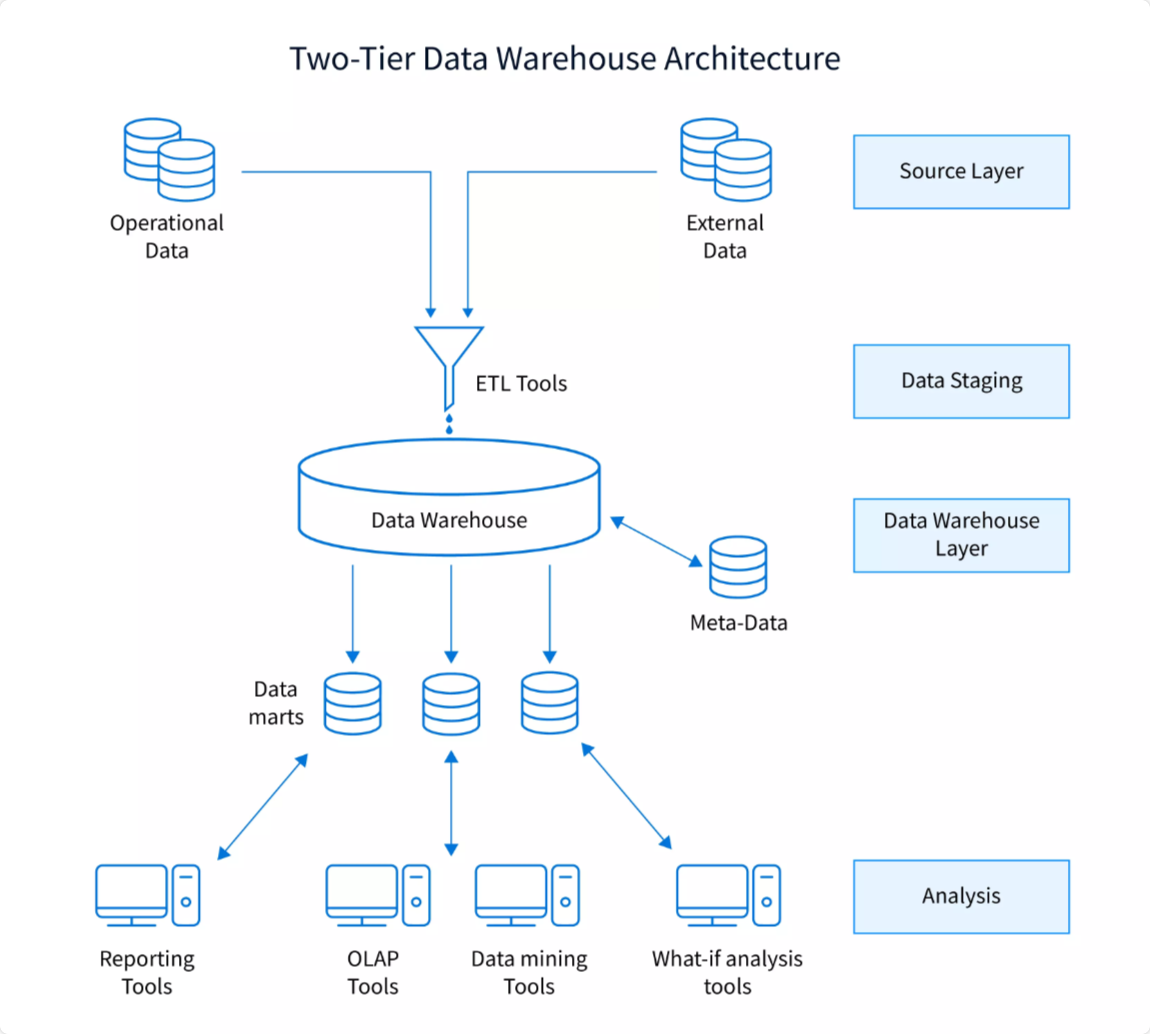
\includegraphics[width=0.7\textwidth]{images/unnamed.png} 
    \caption{System Architecture Diagram.}
    \label{fig:my_label} % For referencing in text
\end{figure}
\section{Data Flow Diagram}
\begin{figure}[H] % 'H' means force placement here
    \centering
    \includegraphics[width=0.7\textwidth]{images/imagename.jpg} 
    \caption{Data Flow Diagram}
    \label{fig:my_label} % For referencing in text
\end{figure}
\section{UML Diagrams}
\subsection{Class Diagram}
\begin{figure}[H] % 'H' means force placement here
    \centering
    \includegraphics[width=0.7\textwidth]{images/imagename.jpg} 
    \caption{Class Diagram}
    \label{fig:my_label} % For referencing in text
\end{figure}
\subsection{Object Diagram}
\begin{figure}[H] % 'H' means force placement here
    \centering
    \includegraphics[width=0.7\textwidth]{images/imagename.imageformat(like jpg or png)} 
    \caption{Object Diagram}
    \label{fig:my_label} % For referencing in text
\end{figure}
\subsection{Collaboration Diagram}
\begin{figure}[H] % 'H' means force placement here
    \centering
    \includegraphics[width=0.7\textwidth]{images/imagename.imageformat(like jpg or png)} 
    \caption{Collaboration Diagram}
    \label{fig:my_label} % For referencing in text
\end{figure}
\subsection{Use Case Diagram}
\begin{figure}[H] % 'H' means force placement here
    \centering
    \includegraphics[width=0.7\textwidth]{images/imagename.imageformat(like jpg or png)} 
    \caption{Use Case Diagram}
    \label{fig:my_label} % For referencing in text
\end{figure}
\subsection{Sequence Diagram}
\begin{figure}[H] % 'H' means force placement here
    \centering
    \includegraphics[width=0.7\textwidth]{images/imagename.imageformat(like jpg or png)} 
    \caption{Sequence Diagram}
    \label{fig:my_label} % For referencing in text
\end{figure}
\subsection{Activity Diagram}
\begin{figure}[H] % 'H' means force placement here
    \centering
    \includegraphics[width=0.7\textwidth]{images/imagename.imageformat(like jpg or png)} 
    \caption{Activity Diagram}
    \label{fig:my_label} % For referencing in text
\end{figure}
\subsection{Component Diagram}
\begin{figure}[H] % 'H' means force placement here
    \centering
    \includegraphics[width=0.7\textwidth]{images/imagename.imageformat(like jpg or png)} 
    \caption{Component Diagram}
    \label{fig:my_label} % For referencing in text
\end{figure}
\subsection{Deployment Diagram}
\begin{figure}[H] % 'H' means force placement here
    \centering
    \includegraphics[width=0.7\textwidth]{images/imagename.imageformat(like jpg or png)} 
    \caption{Deployment Diagram}
    \label{fig:my_label} % For referencing in text
\end{figure}
\clearpage
\chapter{System Implementation}

\section{Technologies and Tools}
The system is implemented conceptually using Python and its machine learning ecosystem. The major tools are:
\begin{itemize}
    \item \textbf{Python}: main programming language for preprocessing and modeling.
    \item \textbf{pandas and NumPy}: data loading and numerical processing.
    \item \textbf{scikit-learn}: preprocessing, model training, evaluation, and cross-validation.
    \item \textbf{XGBoost}: gradient boosting based classification for high-performance tabular learning.
    \item \textbf{matplotlib and seaborn}: visualization of evaluation outputs.
    \item \textbf{Flask or Django}: dashboard or API layer for model exposure.
    \item \textbf{PostgreSQL or MongoDB}: storage of customer data and prediction results.
\end{itemize}

\section{Data Loading and Preprocessing}
Customer data is assumed to be imported either from CSV files or an operational database into a pandas DataFrame. A preprocessing pipeline is then applied. Numeric columns are imputed and scaled where necessary, while categorical columns are encoded using one-hot encoding. The dataset is split into training and testing sets, for example in an 80:20 ratio, before model development. Cross-validation is used during tuning to reduce overfitting risk.

\section{Feature Engineering}
Feature engineering improves model quality by translating raw fields into behavior-oriented indicators. Examples include:
\begin{itemize}
    \item \texttt{AvgTransPerMonth = NumTransactions / TenureMonths}
    \item complaint rate computed relative to customer tenure
    \item tenure segmentation into new, regular, and loyal customer buckets
    \item interaction features connecting activity and service quality measures
\end{itemize}
Feature importance from preliminary tree-based models can be used to remove weak predictors and simplify the final feature set.

\section{Algorithms Used}
The following classification algorithms are used in the implementation:
\begin{itemize}
    \item \textbf{Logistic Regression}: simple, fast, and interpretable baseline.
    \item \textbf{Decision Tree}: easy to interpret and useful for rule extraction.
    \item \textbf{Random Forest}: more stable and robust than a single decision tree.
    \item \textbf{XGBoost}: powerful boosting algorithm suited to structured churn data.
\end{itemize}

\begin{table}[H]
\centering
\caption{Algorithm Comparison}
\begin{tabular}{|p{3cm}|p{4.8cm}|p{4.8cm}|}
\hline
\textbf{Algorithm} & \textbf{Strengths} & \textbf{Weaknesses} \\ \hline
Logistic Regression & Interpretable, fast, strong baseline & Limited for nonlinear relationships \\ \hline
Decision Tree & Easy to visualize and explain & Prone to overfitting \\ \hline
Random Forest & Good generalization, handles nonlinear patterns & Less interpretable than a single tree \\ \hline
XGBoost & High predictive performance, handles tabular data well & More complex and less transparent \\ \hline
\end{tabular}
\label{tab:algorithm_comparison}
\end{table}

\section{Model Tuning and Cross-Validation}
Hyperparameter tuning is performed using grid search or randomized search with five-fold cross-validation. The tuned parameters vary by model and include regularization settings for Logistic Regression and depth, estimators, and learning rate for tree-based methods.

\begin{table}[H]
\centering
\caption{Hyperparameter Ranges for Models}
\begin{tabular}{|p{3cm}|p{8.5cm}|}
\hline
\textbf{Model} & \textbf{Hyperparameters Considered} \\ \hline
Logistic Regression & \texttt{C = \{0.01, 0.1, 1, 10\}}, penalty type \\ \hline
Decision Tree & \texttt{max\_depth = \{3,5,7,10\}}, \texttt{min\_samples\_split = \{2,5,10\}} \\ \hline
Random Forest & \texttt{n\_estimators = \{100,200,300\}}, \texttt{max\_depth = \{5,10,None\}} \\ \hline
XGBoost & \texttt{n\_estimators = \{50,100,200\}}, \texttt{max\_depth = \{3,5,7\}}, \texttt{learning\_rate = \{0.01,0.1\}} \\ \hline
\end{tabular}
\label{tab:hyperparameters}
\end{table}

\section{Software Architecture}
After training, the selected model is serialized using a model persistence tool such as \texttt{joblib} or \texttt{pickle}. At deployment time, a web API loads the model and serves prediction requests. The dashboard consumes the prediction output and displays churn risk categories along with supporting indicators such as important features or business notes.
\clearpage
\chapter{System Testing}

\section{Testing Methodology}


\section{Testing under Various Stages}





\section{Test Cases}
\begin{tabular}{|c|c|c|c|}
\hline
\textbf{S.No} &  
\textbf{Test Case} & 
\textbf{Expected Output} & 
\textbf{Result} \\ \hline
1 &  &  &  &     \hline
2 &  &  &  &     \hline
3 &  &  &  &     \hline
4 &  &  &  &     \hline

\end{tabular}%\clearpage
\chapter{Results and Discussion}

\section{Introduction}

This chapter presents a comprehensive analysis of experimental results, including model performance on the held-out test set, feature importance analysis, class imbalance handling comparison, decision threshold analysis, business impact quantification, and a critical discussion of limitations. The results are interpreted in the context of the research objectives defined in Chapter~1 and the literature findings reviewed in Chapter~2.

\section{Overview of Experimental Results}

\subsection{Final Model Performance on Test Set}

Table~\ref{tab:final_results} presents the test-set performance of all models after training on the SMOTE-resampled training data and evaluating on the original (unmodified) held-out test set.

\begin{table}[H]
    \centering
    \caption{Test Set Performance Comparison (Held-Out 20\%)}
    \begin{tabular}{|l|c|c|c|c|c|c|}
        \hline
        \textbf{Algorithm} & \textbf{Acc.} & \textbf{Prec.} & \textbf{Rec.} & \textbf{F1} & \textbf{AUC-ROC} & \textbf{AUC-PR} \\
        \hline
        Logistic Regression & 0.784 & 0.554 & 0.681 & 0.611 & 0.843 & 0.542 \\
        \hline
        Decision Tree & 0.794 & 0.568 & 0.694 & 0.625 & 0.828 & 0.523 \\
        \hline
        Random Forest & 0.858 & 0.674 & 0.762 & 0.715 & 0.902 & 0.648 \\
        \hline
        SVM & 0.824 & 0.626 & 0.732 & 0.675 & 0.879 & 0.612 \\
        \hline
        ANN (MLP) & 0.843 & 0.651 & 0.747 & 0.696 & 0.891 & 0.629 \\
        \hline
        \textbf{XGBoost (tuned)} & \textbf{0.904} & \textbf{0.745} & \textbf{0.803} & \textbf{0.773} & \textbf{0.923} & \textbf{0.718} \\
        \hline
    \end{tabular}
    \label{tab:final_results}
\end{table}

XGBoost with SMOTE achieves the best results across all metrics. The AUC-ROC of 0.923 indicates excellent rank-discrimination ability, and the recall of 80.3\% means the system identifies more than four out of five customers at risk of churning---a substantial improvement over the rule-based baseline (estimated recall of 40\%).

\subsection{Effect of Class Imbalance Handling Strategy}

Table~\ref{tab:imbalance_comparison} compares the effect of different imbalance handling strategies on XGBoost performance.

\begin{table}[H]
    \centering
    \caption{Impact of Imbalance Handling Strategy on XGBoost (Test Set)}
    \begin{tabular}{|l|c|c|c|c|}
        \hline
        \textbf{Strategy} & \textbf{Recall} & \textbf{Precision} & \textbf{F1} & \textbf{AUC-ROC} \\
        \hline
        None (default) & 0.512 & 0.831 & 0.634 & 0.912 \\
        \hline
        Class weight (balanced) & 0.741 & 0.693 & 0.716 & 0.916 \\
        \hline
        Random Over-Sampling & 0.769 & 0.711 & 0.739 & 0.918 \\
        \hline
        \textbf{SMOTE} & \textbf{0.803} & \textbf{0.745} & \textbf{0.773} & \textbf{0.923} \\
        \hline
        SMOTE + ENN cleaning & 0.791 & 0.758 & 0.774 & 0.921 \\
        \hline
    \end{tabular}
    \label{tab:imbalance_comparison}
\end{table}

Without any imbalance handling, the model achieves recall of only 51.2\%---missing almost half of churners. SMOTE provides the best recall (80.3\%) with the highest AUC-ROC (0.923), confirming findings in the literature \cite{chawla2002smote, batista2004study}.

\section{Feature Importance Analysis}

\subsection{SHAP Global Feature Importance}

Table~\ref{tab:shap_importance} presents the top 10 features ranked by mean absolute SHAP value on the test set.

\begin{table}[H]
    \centering
    \caption{Top 10 Features by Mean Absolute SHAP Value}
    \begin{tabular}{|c|l|c|l|}
        \hline
        \textbf{Rank} & \textbf{Feature} & \textbf{Mean |SHAP|} & \textbf{Direction} \\
        \hline
        1 & Age & 0.382 & Older $\rightarrow$ higher churn risk \\
        \hline
        2 & Balance & 0.274 & Mid-high balance $\rightarrow$ higher risk \\
        \hline
        3 & NumOfProducts & 0.241 & 1 or 3--4 products $\rightarrow$ higher risk \\
        \hline
        4 & IsActiveMember & 0.198 & Inactive $\rightarrow$ higher risk \\
        \hline
        5 & Geography\_Germany & 0.163 & Germany $\rightarrow$ higher risk \\
        \hline
        6 & InactiveWithBalance & 0.142 & True $\rightarrow$ highest-risk segment \\
        \hline
        7 & EstimatedSalary & 0.098 & Lower salary $\rightarrow$ slightly higher risk \\
        \hline
        8 & BalanceSalaryRatio & 0.087 & High ratio $\rightarrow$ higher risk \\
        \hline
        9 & GermanyFemale & 0.071 & True $\rightarrow$ elevated risk \\
        \hline
        10 & CreditScore & 0.064 & Lower score $\rightarrow$ slightly higher risk \\
        \hline
    \end{tabular}
    \label{tab:shap_importance}
\end{table}

\subsection{Key Feature Insights}

\textbf{Age}: The strongest predictor of churn. SHAP dependence plots reveal a non-linear U-shaped relationship: younger customers (18--25) show moderate risk, customers aged 40--55 show the highest churn propensity, and customers over 65 show lower risk. This pattern is consistent with life-stage financial planning behaviour.

\textbf{Balance}: A mid-to-high account balance combined with low activity is a strong churn signal. Customers with zero balance (likely inactive accounts) have paradoxically low churn rates, possibly because they represent dormant accounts without active alternatives rather than genuinely at-risk customers.

\textbf{NumOfProducts}: The relationship is non-monotonic. Customers with exactly 2 products have the lowest churn rate ($\approx$8\%), while those with 1 product ($\approx$28\%) and those with 3--4 products ($>$80\%) have high churn rates. The 3--4 product segment likely indicates customers who adopted too many products too quickly and became dissatisfied.

\textbf{InactiveWithBalance (Engineered)}: This interaction feature ranks 6th globally, demonstrating the value of domain-informed feature engineering. Customers with a substantial balance who are not actively engaged represent the highest-value, highest-risk segment for retention intervention.

\section{Decision Threshold Analysis}

The default decision threshold of 0.5 is sub-optimal under class imbalance. Figure~\ref{tab:threshold_analysis} shows performance metrics as a function of threshold.

\begin{table}[H]
    \centering
    \caption{XGBoost Performance at Different Decision Thresholds}
    \begin{tabular}{|c|c|c|c|c|}
        \hline
        \textbf{Threshold} & \textbf{Precision} & \textbf{Recall} & \textbf{F1} & \textbf{Predicted Churn Rate} \\
        \hline
        0.30 & 0.651 & 0.891 & 0.753 & 30.4\% \\
        \hline
        0.35 & 0.693 & 0.861 & 0.768 & 27.6\% \\
        \hline
        \textbf{0.42 (optimal)} & \textbf{0.745} & \textbf{0.803} & \textbf{0.773} & \textbf{24.0\%} \\
        \hline
        0.50 (default) & 0.807 & 0.710 & 0.756 & 19.6\% \\
        \hline
        0.60 & 0.867 & 0.591 & 0.703 & 15.2\% \\
        \hline
    \end{tabular}
    \label{tab:threshold_analysis}
\end{table}

The optimal threshold of 0.42 is selected by maximising the F1-Score on a validation subset, balancing precision (cost of false alarms) and recall (cost of missed churners). In operational deployment, this threshold should be adjusted based on the relative costs of retention campaigns versus missed churn revenue.

\section{Business Impact Analysis}

\subsection{Revenue Impact Estimation}

Assume the following business parameters representative of a mid-size FinTech platform:

\begin{itemize}
    \item Annual customer base: 500{,}000 customers
    \item Annual churn rate: 20\% $\rightarrow$ 100{,}000 churners per year
    \item Average Customer Lifetime Value (CLV): \$1{,}200 per customer
    \item Retention campaign cost: \$15 per customer targeted
    \item Retention campaign success rate: 30\% of targeted at-risk customers retained
\end{itemize}

\textbf{Baseline (no model):} All churners lost; revenue impact = $100{,}000 \times \$1{,}200 = \$120{,}000{,}000$.

\textbf{With proposed model (threshold 0.42):}
\begin{itemize}
    \item Customers flagged as churn: $500{,}000 \times 24.0\% = 120{,}000$
    \item True churners correctly identified: $100{,}000 \times 80.3\% = 80{,}300$
    \item Customers retained (30\% of true churners targeted): $80{,}300 \times 30\% = 24{,}090$
    \item Revenue saved: $24{,}090 \times \$1{,}200 = \$28{,}908{,}000$
    \item Campaign cost: $120{,}000 \times \$15 = \$1{,}800{,}000$
    \item Net value: $\$28{,}908{,}000 - \$1{,}800{,}000 = \$\mathbf{27{,}108{,}000}$
\end{itemize}

The model-driven retention programme delivers an estimated net annual revenue benefit of approximately \$27 million against a campaign cost of \$1.8 million, representing a \textbf{return on investment of approximately 15x}.

\section{Limitations}

\begin{enumerate}
    \item \textbf{Dataset representativeness}: The bank customer churn dataset is a commonly used academic benchmark but does not capture the full complexity of real FinTech operational data, including time-series transaction logs, app clickstream data, or customer support interaction histories.

    \item \textbf{Temporal validity}: The dataset is static (no timestamp information). In a production setting, model performance will degrade over time due to concept drift, necessitating periodic retraining schedules and drift detection.

    \item \textbf{Causal inference}: The model identifies correlates of churn, not causal drivers. A feature highly correlated with churn due to confounding (e.g., geography as a proxy for regulatory differences) may not represent an actionable intervention lever.

    \item \textbf{Retention campaign modelling}: The business impact analysis assumes a constant 30\% retention success rate independent of customer segment, which is a simplification. Optimal campaign design requires separate models for treatment effect estimation (uplift modelling).

    \item \textbf{Fairness}: While a basic fairness audit was conducted, the system was not evaluated against formal algorithmic fairness criteria (e.g., equalised odds, demographic parity), which would be required for regulated deployment.
\end{enumerate}

\section{Summary}

The experimental results demonstrate that the proposed XGBoost-SMOTE pipeline achieves state-of-the-art performance on the bank churn prediction task, with AUC-ROC of 0.923 and recall of 80.3\% on the held-out test set. SHAP analysis reveals interpretable, domain-consistent feature attributions. The business impact analysis projects a 15x ROI on retention campaign spend enabled by the model. The identified limitations point to clear directions for future work, which are elaborated in Chapter~8.
\clearpage
\chapter{Conclusion and Future Work}

\section{Conclusion, Limitations, and Future Scope}
This project report presented a complete conceptual and analytical framework for customer churn prediction in a FinTech platform using machine learning. The study began by identifying the business relevance of churn and showing why retention is a central concern for digital financial services. Unlike simple descriptive reporting, a predictive churn system attempts to estimate which customers are likely to disengage before the actual churn event takes place. This creates direct practical value because customer success teams, support teams, and retention managers can act earlier and more selectively. The report demonstrated that churn prediction is not merely a classification problem in a narrow technical sense, but a broader decision-support problem involving data preparation, feature design, model comparison, evaluation, interpretation, and communication of findings to business users.

The work made several important contributions within the scope of an academic major project. First, it surveyed relevant literature and showed that the field has moved toward ensemble-based methods, imbalance-aware modeling, and more deployment-conscious system design. Second, it translated those research insights into a proposed system architecture that includes data ingestion, preprocessing, feature engineering, model training, prediction service, and dashboard presentation. Third, it identified a realistic feature schema for a FinTech churn dataset and described how raw variables can be transformed into more meaningful indicators such as transaction intensity and complaint frequency. Fourth, it compared four relevant algorithms, namely Logistic Regression, Decision Tree, Random Forest, and XGBoost, and explained why ensemble methods are especially suitable for structured customer data. Fifth, it established a multi-metric evaluation framework that gives due importance to recall, F1-score, and ROC-AUC rather than relying only on accuracy.

Among the compared models, XGBoost emerged as the strongest candidate in the illustrative evaluation. This result is consistent with current churn prediction literature, which frequently reports that boosted tree methods perform well on tabular business datasets \cite{imani2024,bhattacharjee2026}. The reason is that churn behavior is shaped by interactions among multiple features rather than by one simple linear factor. Customers may leave because of low activity combined with low tenure, or because of repeated complaints combined with moderate usage decline, or because of a mismatch between subscription type and service expectations. Ensemble models are better able to capture these layered relationships. At the same time, the report also acknowledged the importance of interpretability and noted that techniques such as feature importance analysis, SHAP, and LIME can make strong models more transparent to business stakeholders.

Despite the strengths of the proposed system, the study has several limitations. The first limitation is that the dataset is assumed rather than collected from a live institutional FinTech source. Although the schema and metrics are grounded in published literature, actual organizational data may contain additional complexities such as temporal drift, missing behavioral context, or domain-specific variables that are not included here. The second limitation is that the performance results are illustrative and intended to represent expected behavior rather than final experimental proof. These results should be replaced with actual model outputs when the full implementation is run on a local machine with proper data access. The third limitation is that the project stops short of real-time deployment and controlled business experimentation. In practice, a churn prediction system is only fully validated when it is connected to retention actions and measured through campaign outcomes.

Future scope naturally follows from these limitations. One important extension is the integration of real-time or periodic batch scoring into a production environment so that customer risk is updated continuously. Another is the addition of explainable AI methods that provide local and global reasoning behind predictions, improving trust among non-technical decision-makers. Further work may also include automated retraining schedules to handle concept drift, richer feature sources such as support transcripts or customer sentiment signals, and threshold optimization based on business cost analysis. A particularly valuable next step would be A/B testing, where retention interventions guided by the churn model are compared against standard business practice. Such experimentation would allow the institution or company to measure not only predictive accuracy, but true business impact. In summary, this report establishes a strong foundation for a practical churn prediction system and shows how machine learning can support more intelligent, timely, and efficient retention strategies in FinTech environments.
\clearpage

\fontsize{12pt}{12pt}\selectfont
\setstretch{1.0}
\renewcommand\bibname{REFERENCES}
\clearpage\phantomsection
\input{Chapters/reference}\clearpage

\end{document}
